\chapter{Critical Evaluation}

In this chapter, I describe the set of experiments used to show the increase in performance from the implementation of the constraint-based approach. \\ \\
I have measured the performance by running both versions of the learner on five target problems, and returning both the generated code and the time taken to learn, as returned by clingo. The problems are defined by a set of Input / Output examples which cover enough cases to correctly learn the target function. Solutions are defined as a subset of the generated Answer Set, containing only \lstinline{choose}, \lstinline{choose_match} and \lstinline{choose_where} atoms, representing chosen rules from the skeleton rules. \\ \\%{ 
The five examples I am running are defined as follows.
\begin{itemize}
\item \textbf{Factorial} : The recursive definition of the mathematical factorial operation, denoted by \lstinline{n!} . It is defined as the product of all positive integers less than or equal to \lstinline{n}.% {
\item \textbf{Fibonacci} : The Fibonacci numbers belong to the following sequence - \lstinline{1, 1, 2, 3, 5, 8, 13}, where each member of the sequence is equal to the sum of the previous two numbers. %{
\item \textbf{Powers of Two} : A simple function which recursively defines the calculation of $2^n$.
\item \textbf{Tail Recursive Factorial} : The tail-recursive definition of the factorial function. Takes two arguments, where the second is an accumulator in which the product is calculated.
\item \textbf{Greatest Common Divisor} : A version of Euclid's algorithm to calculate the greatest common divisor of two numbers.
\end{itemize}
All examples have been run on --LAB PC SPECS-- \\ \\

\pagebreak

\section{Generated Code}

\subsection{Factorial}
\underline{\textbf{Input Examples}}
\begin{lstlisting}
example(call(fac, 0), 1).
example(call(fac, 1), 1).
example(call(fac, 2), 2).
example(call(fac, 3), 6).
\end{lstlisting}

\begin{multicols}{2}

\underline{\textbf{Interpreted approach results}}
\begin{lstlisting}
fac x
  | x == 0 = 1
  | otherwise = x * x0
  where x0 = f x1
  	where x1 = x - 1
\end{lstlisting}
%\vspace*{\fill}
\columnbreak
\underline{\textbf{Constraint approach results}}
\begin{lstlisting}
fac x
  | x == 0 = 1
  | otherwise = (fac (x - 1)) * x
\end{lstlisting}
\end{multicols}

\subsection{Fibonacci}
\underline{\textbf{Input Examples}}
\begin{lstlisting}
example(call(f, 1), 1).
example(call(f, 2), 1).
example(call(f, 3), 2).
example(call(f, 4), 3).
example(call(f, 5), 5).
example(call(f, 6), 8).
\end{lstlisting}

\begin{multicols}{2}
\underline{\textbf{Interpreted approach results}}
\begin{lstlisting}
fib x
  | x == 1 = x
  | x == 2 = x - 1
  | otherwise = x0 + x2
  where x0 = fib x1
  	where x1 = x - 1
  		where x2 = fib x3
  			where x3 = x - 2
\end{lstlisting}
%\vspace*{\fill}
\columnbreak
\underline{\textbf{Constraint approach results}}
\begin{lstlisting}
UNSATISFIABLE
\end{lstlisting}
\end{multicols}

\pagebreak
\subsection{Powers of 2}
\underline{\textbf{Input Examples}}
\begin{lstlisting}
example(call(f, 0), 1).
example(call(f, 1), 2).
example(call(f, 2), 4).
example(call(f, 3), 8).
\end{lstlisting}

\begin{multicols}{2}
\underline{\textbf{Interpreted approach results}}
\begin{lstlisting}
power2 x
  | x == 0 = x + 1
  | otherwise = x1 + x2
  	where x1 = f x0
  		where x2 = f x0
  			where x0 = x - 1
\end{lstlisting}
%\vspace*{\fill}
\columnbreak
\underline{\textbf{Constraint approach results}}
\begin{lstlisting}
power2 x
  | x == 1 = 1
  | otherwise = (f (x - 1)) * 2 
\end{lstlisting}
\end{multicols}

\subsection{Tail Recursive Factorial}
\underline{\textbf{Input Examples}}
\begin{lstlisting}
example(call(f, (0, 1)), 1).
example(call(f, (1, 1)), 1).
example(call(f, (2, 1)), 2).
example(call(f, (3, 1)), 6).
example(call(f, (2, 3)), 6).
\end{lstlisting}

\begin{multicols}{2}
\underline{\textbf{Interpreted approach results}}

\begin{lstlisting}
fac x y
  | x == 0 = y
  | otherwise = fac x0 x1
  where x0 = x - 1
  	where x1 = x * y
\end{lstlisting}
%\vspace*{\fill}
\columnbreak
\underline{\textbf{Constraint approach results}}
\begin{lstlisting}
fac x y
  | x == 0 = y
  | otherwise = fac (x - 1) (x * y)
\end{lstlisting}
\end{multicols}
%\pagebreak
\pagebreak
\subsection{Greatest Common Divisor}
\underline{\textbf{Input Examples}}
\begin{lstlisting}
example(call(gcd, (1, 1)), 1).
example(call(gcd, (2, 1)), 1).
example(call(gcd, (4, 3)), 1).
example(call(gcd, (3, 6)), 3).
example(call(gcd, (9, 6)), 3).
example(call(gcd, (4, 7)), 1).
example(call(gcd, (9, 3)), 3).
\end{lstlisting}
\begin{multicols}{2}
\underline{\textbf{Interpreted approach results}}
\begin{lstlisting}
gcd x y
  | y == 0 = x
  | x > y = gcd y x0
  | otherwise = gcd x1 x
  where x0 = x - y
  	where x1 = y - x
\end{lstlisting}
\vspace*{\fill}
\columnbreak
\underline{\textbf{Constraint approach results}}
\begin{lstlisting}
gcd x y
	| x == y = x
	| x > y	 = gcd (x - y) y
	| x < y	 = gcd y x
\end{lstlisting}
\end{multicols}

\section{Performance Statistics}
The results from these experiments tend to show the result that apart from in the simple case, the constraint based approach performs around 50\% better than the interpreted approach across all examples. In the simple factorial example, the interpreted approach was quicker due to the small set of skeleton rules effecting performance in relatively small way. \\ \\
The one case where the constraint based approach performs worse to the interpreted approach is the GCD example. While it is not clear why this is the case, it is most likely due to the way skeleton rules are generated. Due to the need to enumerate over all possible skeleton rules in the constraint based approach, this means that many rules could be semantically equal to each other, reducing performance in this case. This effect only appears here as the number of skeleton rules needed to correctly learn gcd is much higher than the other functions. \\ \\
However, the constraint based approach is less expressive, as highlighted by the fibonacci example. The fibonacci program consists of two recursive calls, which cannot be learned by this approach as it becomes difficult to maintain the equality constraints. For example, consider the equality constraint \lstinline{eq(add(call(f, (x - 1)), call(f, (x - 2))), 4).} The tool cannot continue evaluating this constraint as it does not know the value of either \lstinline{call} expressions.%{

\pagebreak

\begin{table}[h!]
\centering
\begin{tabular}{|c|m{10em}|m{10em}|}
\hline
\multicolumn{3}{|c|}{\textbf{Performance}}\\
\hline
Function & Interpreted  & Constraint Based \\
\hline
Factorial 
& 
\mbox{}\newline
Time        : 1.640 \newline
  Prepare   : 0.060 \newline
  Prepro.   : 0.020 \newline
  Solving   : 1.560 \newline
& 
\mbox{}\newline
Time        : 1.240 \newline
  Prepare   : 0.200 \newline
  Prepro.   : 0.140 \newline
  Solving   : 0.900 \newline
\\
\hline
Fibonacci 
&
\mbox{}\newline 
Time        : 807.240 \newline
  Prepare   : 0.060 \newline
  Prepro.   : 0.020 \newline
  Solving   : 807.160 \newline
& 
Unsatisfiable
\\
\hline
Power of Two 
&
\mbox{}\newline 
Time        : 35.840 \newline
  Prepare   : 0.040 \newline
  Prepro.   : 0.040 \newline
  Solving   : 35.760 \newline
& 
\mbox{}\newline 
Time        : 5.580 \newline
  Prepare   : 0.380 \newline
  Prepro.   : 0.340 \newline
  Solving   : 4.860 \newline
\\
\hline
Tail Recursive Factorial
&
\mbox{}\newline 
Time        : 419.860 \newline
  Prepare   : 2.060 \newline
  Prepro.   : 0.840 \newline
  Solving   : 416.960 \newline
& 
\mbox{}\newline 
Time        : 173.900 \newline
  Prepare   : 5.540 \newline
  Prepro.   : 1.440 \newline
  Solving   : 166.920 \newline
\\
\hline
GCD 
& 
\mbox{}\newline 
Time        : 1546.820 \newline
  Prepare   : 1.940 \newline
  Prepro.   : 0.980 \newline
  Solving   : 1543.900 \newline
& 
\mbox{}\newline 
Time        : 1599.420 \newline
  Prepare   : 11.720 \newline
  Prepro.   : 2.100 \newline
  Solving   : 1585.600 \newline
\\
\hline
\end{tabular}
\caption{Approach Performance Comparison }
\label{table:3}
\end{table}

\pagebreak
\section{Comparison to Existing Tools}

In this section, I will detail how other existing inductive functional programming (IFP) tools perform in comparison to mine, highlighting any benefits or restrictions to both mine and the existing tools. More information on these tools can be found in the background section. \\ \\
For evaluation, I have ran both systems on the examples detailed in the section above, showing a comparison between code generated and running time between both existing systems and my tool's constraint based approach.

\subsection{MagicHaskeller}
MagicHaskeller \cite{Katayama2012} is an IFP system that is based on the generate-and-test approach to IFP. It works by systematically generating a stream of gradually more complicated functions (based on length), and keeping the ones which cover the input examples. \\ \\
Input to MagicHaskeller is any Haskell expression which returns a boolean value, as long as it does not contain any \lstinline{let} or \lstinline{while} clauses. For example, to learn the factorial program, you can give as input the examples \lstinline{\f -> ( f 0 == 1 )  && ( f 1 == 1 )  && ( f 2 == 2 )  && ( f 3 == 6 )}. Here, each positive example is concatenated with \lstinline{&&} to produce the overall input.\\ \\
Full tables of generated programs and performance timings can be found respectively in Tables \ref{table:1} and \ref{table:2} \\ \\
What is notable from these results is that MagicHaskeller fails to learn direct recursion, relying instead on its large library of in-built functions. This is most visible on the GCD and Fibonacci examples, where MagicHaskeller can simply make use of Haskell's inbuilt gcd function, but cannot learn the purely recursive Fibonacci. This is because of a deliberate choice by the creator of MagicHaskeller, as removing direct recursion decreases the complexity of the search space.

\begin{figure}[h!]
\centering
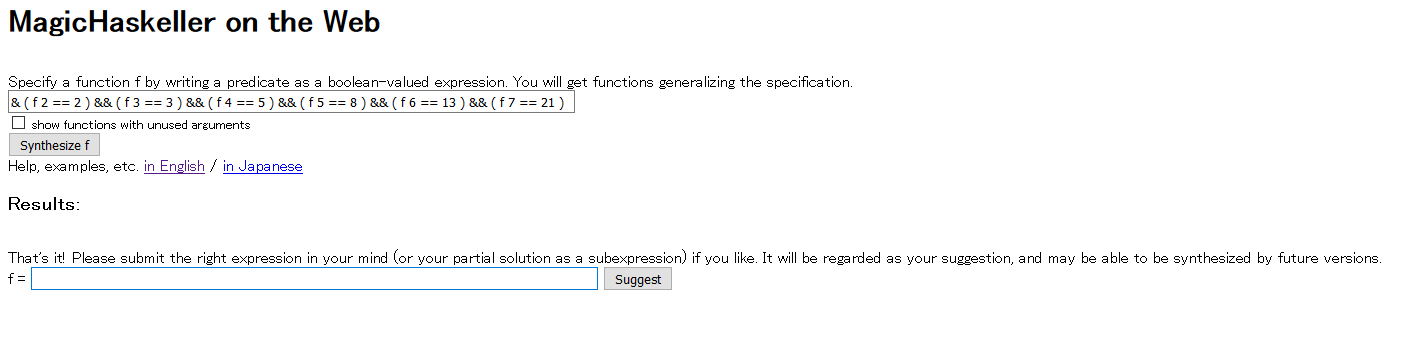
\includegraphics[width=\textwidth]{C7/magichaskeller_fail.png}
\caption{MagicHaskeller fibonacci attempt}
\label{fig:magichaskeller_fail}
\end{figure}

\Suppressnumber

\begin{table}[h!]
\centering
\begin{tabular}{| m{4em} | c | c |}
\hline
\multicolumn{3}{|c|}{\textbf{Generated Code}} \\
\hline
Function & My Solution & MagicHaskeller Solution \\
\hline
Factorial 
&
\begin{lstlisting}[backgroundcolor = \color{white}]
f x
  | x == 0 = 1
  | otherwise = x * f(x - 1)
\end{lstlisting}
& 
\begin{lstlisting}[backgroundcolor = \color{white}]
f = 
  (\a -> product [1..a])
\end{lstlisting}
\\
\hline
\mbox{}\newline
Power \newline
of \newline
Two \newline
&
\mbox{}\newline
\begin{lstlisting}[backgroundcolor = \color{white}]
f x
  | x == 0 = 1
  | otherwise = 2 * f(x - 1)
\end{lstlisting}
& 
\begin{lstlisting}[backgroundcolor = \color{white}]
f = 
  (\a -> product (replicate a 2))
\end{lstlisting}
\\
\hline
\mbox{}\newline
Tail \newline
Recursive \newline
Factorial \newline
&
\begin{lstlisting}[backgroundcolor = \color{white}]
f x n
  | x == 0 = n
  | otherwise = f (x - 1) (x * n)
\end{lstlisting}
& 
\begin{lstlisting}[backgroundcolor = \color{white}]
f = 
  (\a b -> product [b..a])
\end{lstlisting}
\\
\hline
GCD 
&
\begin{lstlisting}[backgroundcolor = \color{white}]
gcd x y
  | x == y = x
  | x > y  = gcd x - y y
  | x < y  = gcd y x
\end{lstlisting}	
&
\begin{lstlisting}[backgroundcolor = \color{white}]
f = (flip gcd)
\end{lstlisting}
\\
\hline
Fibonacci
&
\begin{lstlisting}[backgroundcolor = \color{white}]
fib x
  | x == 1 = x
  | x == 2 = x - 1
  | otherwise = x0 + x2
  where x0 = fib x1
  	where x1 = x - 1
  		where x2 = fib x3
  			where x3 = x - 2
\end{lstlisting}
&
No Result!
\\
\hline
\end{tabular}
\caption{MagicHaskeller Generated Code Comparison }
\label{table:1}
\end{table}
\Reactivatenumber

\begin{table}[h!]
\centering
\begin{tabular}{|c|c|c|}
\hline
\multicolumn{3}{|c|}{\textbf{Performance}}\\
\hline
Function & My Performance & MagicHaskeller \\
\hline
Factorial & & \\
\hline
Tail Recursive Factorial & & \\
\hline
GCD & & \\
\hline
Fibonacci & & \\
\hline
\end{tabular}
\caption{MagicHaskeller Performance Comparison }
\label{table:2}
\end{table}

\subsection{Igor II}
Igor II \cite{Kitzelmann2006} is an IFP system that is designed to learn purely recursive programs, and is different to the tool described in this report in important ways.
\begin{itemize}
\item Igor II does not have any built in background knowledge, which means that any functions to be learned need all basic operations and constants defined at the same time as the examples. This is only a small restriction for learning lists because the set of constants and operations to be defined are limited to the empty list and list prepending respectively. However, when learning arithmetic functions it is very complicated to define addition and multiplication in terms of the basic succession operation.
\item The output from Igor II is a list of hypotheses, rather than a program or lambda function. While this increases the expressivity, it severely reduces readability and usability by users less experienced in the field.
\end{itemize}


\pagebreak
%\renewcommand\bibname{{References}}
%\bibliography{References}
%\bibliographystyle{plain}